\documentclass[conference]{IEEEtran}
% correct bad hyphenation here
\hyphenation{op-tical net-works semi-conduc-tor}

%%%%%%%%%%%%%%%%%%%%%%%%%%%%%%%%%%%%%%%%%%%%%%%%%%%%
\usepackage{lineno,hyperref}
\usepackage{amsmath}
\usepackage{graphicx}
\usepackage{tabularx}
\usepackage[usenames, dvipsnames]{color}
\usepackage{rotating}
\usepackage{caption}
\captionsetup{font={small}} 
%\usepackage[english]{babel}
%\usepackage[utf8]{inputenc}
%\usepackage[T1]{fontenc}
%\usepackage{lmodern}
%\usepackage[table]{xcolor}
%\usepackage{hyperref} % must be loaded before glossaries-extra
% bibliography
%\usepackage[hyperref=true,backref=true,backend=biber,maxbibnames=9,maxcitenames=2,style=numeric,citestyle=numeric,sorting=none]{biblatex} % hyperref uses links, backref goes back to citations, uses biber as backend, with 9 names at most in bibliography and 2 in citations, citing using numbers, and sorting in citation order
% sorting can be also ydnt for year descending, name, title or ynt for ascending year

%\usepackage{adjustbox} % to resize boxes by keeping the same aspect ratio
\usepackage{algorithm} % algorithm environment
\usepackage{algpseudocode} % improved pseudo-code
%\usepackage{amsfonts}               %  AMS mathematical fonts
%\usepackage{amsmath}
%\usepackage{amssymb}                %  AMS mathematical symbols
%\usepackage{bm}                     %  black/bold mathematical symbols
%\usepackage{booktabs}               %  better tables
%\usepackage[labelfont=bf]{caption} % font=footnotesize % to have reduced caption font size
%\usepackage{csquotes}
\usepackage{enumitem} %left align the bulleted points
%\usepackage{geometry}
%\usepackage{glossaries} % to use acronyms and glossary, it has also glossaries-extra as extension, but commands are different
% \usepackage[%
%     toc, % puts the link in the ToC
%     %record, % to use bib2gls
%     abbreviations, % to load abbreviations / acronyms
%     nonumberlist, % to avoid printing the numbers of the references in the acronyms page
% ]{glossaries-extra}
% \usepackage{graphicx}               %  post-script images
% %\usepackage{iwona} % extra fonts, substitute standard ones
% \usepackage{listings} % to insert formatted code
% %\usepackage{lipsum} % for lorem ipsum text, not needed in the real work
% \usepackage{makecell} % to change dimensions of cells, for math cases
% \usepackage{mathtools} % for additional commands
% \usepackage{mfirstuc} % to have capitalization capabilities
% \usepackage[final]{microtype}      % microtypography, final lets latex use it also in bibliography
% \usepackage{multirow} % to allow for cells covering more than 1 row in tables
% \usepackage{nicefrac}       % compact symbols for 1/2, etc.
% %\usepackage[lofdepth,lotdepth]{subfig}
% \usepackage{ragged2e} % for justifying text
% \usepackage{siunitx} % support for SI units of measurement and number typesetting
% \usepackage{subfig}
% \usepackage{svg} % for svg support, works only if inkscape is installed, default for Overleaf v2
% %\usepackage{subfigure}              %  subfigure compatibility, can be removed if subfig
% \usepackage{tabularx} % equal-width columns in tables
% \usepackage{textcomp} % extra fonts and symbols
% \usepackage{url}            % simple URL typesetting
% \usepackage{verbatim} % for extended verbatim support
% \usepackage{xcolor} % to define colors and use standard CSS names add dvipsnames as option, but it clashes with xcolor loaded in toptesi, pay attention that if it goes in conflict with tikz/beamer, simply use \documentclass[usenames,dvipsnames]{beamer}, along with other custom options when defining the document class
\usepackage{algorithmicx}
%%%% added by gianluca
\providecommand{\com}[1]{{\color{red}\emph{#1}}}
\newcommand{\fref}[1]{Fig.~\ref{#1}}
%create notation table
\linespread{1.09}
%\usepackage[labelfont=bf,format=plain,justification=raggedright,singlelinecheck=false]{caption}
%% configuration for glossaries
% convert and load converted glossaries in .tex ,format from .bib
\setabbreviationstyle{long-short-desc} % style before loading resources
% this command sets the style to title for long names of acronyms only in the glossary description, leading to capitalized first-letter for all words
% \glssetcategoryattribute{\glsxtrabbrvtype}{glossname}{capitalisewords} % doesn't work
% resources to load if using a bib file with bib2gls
%\GlsXtrLoadResources[%
% src={glossaries}, % name of the file without extension
% selection=all, % select all the entries
%]
% not needed
%\newglossary*{abbreviation}{Acronyms} % to change the name of this glossary for acronyms

%\renewcommand{\glsclearpage}{\paginavuota} % to allow glossaries to clear pages, done manually is better


% setup for hyperref
\hypersetup{%
    pdfpagemode={UseOutlines},
    bookmarksopen,
    pdfstartview={FitH},
    colorlinks,
    linkcolor={black}, % it is suggested to keep them black, since when printing it it costs per page, and if they have color it's twice the price per page
    citecolor={black},
    urlcolor={black}
  }
%

% setup for svg
\svgsetup{%
    inkscapeformat=pdf, % to force usage of PDF
    inkscapelatex=false, % to disable latex rendering of text, produces errors
}

% setup for siunitx, it does not work in the summary
\sisetup{%
    detect-all, % to use the same font as for writing when using \num
    mode=text, % to allow it to work also in math mode
    group-separator = {,}, % separator for number grouping
    group-minimum-digits = 3, % minimum number of digits a number must have to be grouped in 3-digit groups
}

% listings colours
\definecolor{rulecolor}{rgb}{0,0,0}
\definecolor{commentcolor}{rgb}{0,0.6,0}
\definecolor{linenumbercolor}{rgb}{0.5,0.5,0.5}
\definecolor{keywordcolor}{rgb}{0,0,0.95}
\definecolor{backcolor}{rgb}{1,1,1}%{0.95,0.95,0.92}
\definecolor{stringcolor}{rgb}{0.58,0,0.82}

% setup for lstlisting
\lstset{ %
	backgroundcolor=\color{backcolor},   % choose the background color; you must add \usepackage{color} or \usepackage{xcolor}; should come as last argument
	basicstyle=\footnotesize,        % the size of the fonts that are used for the code
	breakatwhitespace=false,         % sets if automatic breaks should only happen at whitespace
	breaklines=true,                 % sets automatic line breaking
	captionpos=t,                    % sets the caption-position to bottom
	commentstyle=\color{commentcolor},    % comment style
	extendedchars=true,              % lets you use non-ASCII characters; for 8-bits encodings only, does not work with UTF-8
	frame=single,	                   % adds a frame around the code
	keepspaces=true,                 % keeps spaces in text, useful for keeping indentation of code (possibly needs columns=flexible)
	keywordstyle=\color{keywordcolor},       % keyword style
	%language=VHDL,                 % the language of the code
	numbers=left,                    % where to put the line-numbers; possible values are (none, left, right)
	numbersep=5pt,                   % how far the line-numbers are from the code
	numberstyle=\tiny\color{linenumbercolor}, % the style that is used for the line-numbers
	rulecolor=\color{rulecolor},         % if not set, the frame-color may be changed on line-breaks within not-black text (e.g. comments (green here))
	showspaces=false,                % show spaces everywhere adding particular underscores; it overrides 'showstringspaces'
	showstringspaces=false,          % underline spaces within strings only
	showtabs=false,                  % show tabs within strings adding particular underscores
	stepnumber=1,                    % the step between two line-numbers. If it's 1, each line will be numbered
	stringstyle=\color{stringcolor},     % string literal style
	tabsize=4,	                   % sets default tabsize to 2 spaces
	title=\lstname,                   % show the filename of files included with \lstinputlisting; also try caption instead of title
	inputencoding=utf8,
	literate=
	{á}{{\'a}}1 {é}{{\'e}}1 {í}{{\'i}}1 {ó}{{\'o}}1 {ú}{{\'u}}1
	{Á}{{\'A}}1 {É}{{\'E}}1 {Í}{{\'I}}1 {Ó}{{\'O}}1 {Ú}{{\'U}}1
	{à}{{\`a}}1 {è}{{\`e}}1 {ì}{{\`i}}1 {ò}{{\`o}}1 {ù}{{\`u}}1
	{À}{{\`A}}1 {È}{{\'E}}1 {Ì}{{\`I}}1 {Ò}{{\`O}}1 {Ù}{{\`U}}1
	{ä}{{\"a}}1 {ë}{{\"e}}1 {ï}{{\"i}}1 {ö}{{\"o}}1 {ü}{{\"u}}1
	{Ä}{{\"A}}1 {Ë}{{\"E}}1 {Ï}{{\"I}}1 {Ö}{{\"O}}1 {Ü}{{\"U}}1
	{â}{{\^a}}1 {ê}{{\^e}}1 {î}{{\^i}}1 {ô}{{\^o}}1 {û}{{\^u}}1
	{Â}{{\^A}}1 {Ê}{{\^E}}1 {Î}{{\^I}}1 {Ô}{{\^O}}1 {Û}{{\^U}}1
	{œ}{{\oe}}1 {Œ}{{\OE}}1 {æ}{{\ae}}1 {Æ}{{\AE}}1 {ß}{{\ss}}1
	{ű}{{\H{u}}}1 {Ű}{{\H{U}}}1 {ő}{{\H{o}}}1 {Ő}{{\H{O}}}1
	{ç}{{\c c}}1 {Ç}{{\c C}}1 {ø}{{\o}}1 {å}{{\r a}}1 {Å}{{\r A}}1
	{€}{{\euro}}1 {£}{{\pounds}}1 {«}{{\guillemotleft}}1
	{»}{{\guillemotright}}1 {ñ}{{\~n}}1 {Ñ}{{\~N}}1 {¿}{{?`}}1
}


% % biblatex setup
% % generally 9000 is ok, if higher than 10000 it's bad
% % If you want to break on URL numbers
% \setcounter{biburlnumpenalty}{9000}
% % If you want to break on URL lower case letters
% \setcounter{biburllcpenalty}{9000}
% % If you want to break on URL UPPER CASE letters
% \setcounter{biburlucpenalty}{9000}

%
% % how to change Contents to Table of Contents
% \addto\captionsenglish{% Replace "english" with the language you use
%   \renewcommand{\contentsname}%
%     {Table of Contents}%
% }

% to change the name of Abbreviations to Acronyms
% not needed if use use entry types and define those
% \renewcommand{\abbreviationsname}{Acronyms}

% to allow line comments in algorithms
\algnewcommand{\LineComment}[1]{\State \(\triangleright\) #1}

% to declare abs and norm
\DeclarePairedDelimiter\abs{\lvert}{\rvert}%
\DeclarePairedDelimiter\norm{\lVert}{\rVert}%

% Swap the definition of \abs* and \norm*, so that \abs
% and \norm resizes the size of the brackets, and the 
% starred version does not.
\makeatletter
\let\oldabs\abs
\def\abs{\@ifstar{\oldabs}{\oldabs*}}
%
\let\oldnorm\norm
\def\norm{\@ifstar{\oldnorm}{\oldnorm*}}
\makeatother

\pagestyle{plain}
\DeclareMathOperator*{\argmin}{arg\,min}
%figure


% \makeatletter
% \def\Cline#1#2{\@Cline#1#2\@nil}
% \def\@Cline#1-#2#3\@nil{%
%   \omit
%   \@multicnt#1%
%   \advance\@multispan\m@ne
%   \ifnum\@multicnt=\@ne\@firstofone{&\omit}\fi
%   \@multicnt#2%
%   \advance\@multicnt-#1%
%   \advance\@multispan\@ne
%   \leaders\hrule\@height#3\hfill
%   \cr}
% \makeatother

\begin{document}
%
% paper title
% Titles are generally capitalized except for words such as a, an, and, as,
% at, but, by, for, in, nor, of, on, or, the, to and up, which are usually
% not capitalized unless they are the first or last word of the title.
% Linebreaks \\ can be used within to get better formatting as desired.
% Do not put math or special symbols in the title.

%Feasibility of Floating Content modeling through a variation of Random Waypoint
%\title{Gossip Learning: Personalized Models \\
%for Vehicle Trajectory Prediction \vspace{-0.3in}}
\title{Gossip Learning of Personalized Models \\
for Vehicle Trajectory Prediction \vspace{-0.3in}}

\vspace{-65pt}
% author names and affiliations
% use a multiple column layout for up to three different
% affiliations
\author{\IEEEauthorblockN{Mina Aghaei Dinani,\\Adrian Holzer}
\IEEEauthorblockA{University of Neuchatel,\\ Switzerland\\name.surname@unine.ch}
\and
\IEEEauthorblockN{Hung Nguyen}
\IEEEauthorblockA{The University of Adelaide,\\ Australia\\hung.nguyen@adelaide.edu.au}
\and
\IEEEauthorblockN{Marco Ajmone Marsan}
\IEEEauthorblockA{Politecnico di Torino, Italy and\\ Institute IMDEA Networks, Spain\\ajmone@polito.it}
\and
\IEEEauthorblockN{Gianluca Rizzo}
\IEEEauthorblockA{HES-SO Valais, Switzerland, and\\
University of Foggia, Italy
\\gianluca.rizzo@hevs.ch}
}


% make the title area
\maketitle

% creates the second title. It will be ignored for other modes.
%\IEEEpeerreviewmaketitle
\begin{abstract} 
%Increasing concerns on user privacy, the growing pervasiveness of sensing and distributed data generation, and the rise in computing demand at the edge of the network are calling for a shift in paradigm towards fully decentralized machine learning approaches, which guarantee better scalability and privacy protection trhan traditional, centralized architectures. In this context, a special role is played by Gossip Learning (GL), a peer-to-peer machine learning protocol based on direct, opportunistic exchange of models among nodes via wireless D2D communications, and on collaborative model training, which has recently proven to scale efficiently to large number of nodes.
%employs a client-server architecture with each node acting as client and server, possibly at the same time. GL is not based on a central server and is therefore highly scalable. Each node exchanges local model instance with neighbors, Neighbors train received models based on their local dataset and send partially trained model back,with no raw data exposure, so that user privacy is preserved.
%Nodes train their own model instance based on their local dataset, and exchange model instances with neighbors, with no raw data exposure, so that user privacy is preserved.\\
Gossip Learning (GL) is a peer-to-peer machine learning protocol based on direct, opportunistic exchange of models among nodes via wireless D2D communications, and on collaborative model training, which has recently proven to scale efficiently to large numbers of nodes, and to offer better privacy guarantees than traditional centralized learning architectures.
Existing approaches to GL are however limited to scenarios in which nodes are static, or in which the node connectivity graph is fully connected, and they are fragile to node churn as well as to any change in network configuration. 
%It is thus so far unclear how to apply them in realistic, dynamic setups where nodes join and leave the network, such as in vehicular ad-hoc networks (VANETs).\\
To overcome this limitation, we present a new decentralized architecture for GL suitable for setups with dynamic nodes,  which benefits from node mobility instead of being hampered by it. In our approach, nodes improve their personalized model instance by sharing it with neighbors, and by weighting neighbors' contributions according to an estimate of their marginal utility. % Hence, as many local consensus models are developed as the number of nodes.\\
We apply our GL algorithm to short-term vehicular trajectory estimation in realistic urban scenarios. %Specifically, we assume that data is unevenly distributed across vehicles, and that \com{no vehicle obtains a representative sample of the model instances available in the overall population.}
%(ii) each vehicle only collects a tiny fraction of the data produced by the whole , and (iii) no vehicle obtains a representative sample of the model instances available in the overall population. 
We propose a new strategy for the estimation of the neighbors' instances marginal utility, which yields satisfactory trajectory estimation accuracy for nodes with long enough sojourn times.

%Then we define three  practical gossip learning algorithms called DFed Avg, DFed Pow, and DFed Best. We applied an LSTM model on a dynamic time series dataset while connectivity graph amongst nodes is not static.\\
%Numerical evaluations show that these approaches perform well in dynamic scenarios, with high accuracy () and low loss (). %particularly when vehicles spend an adequately amount of time (min 20 min).
 \end{abstract}

\vspace{-15pt}
\section{Introduction}
\vspace{-5pt}
% no \IEEEPARstart
The amount of data produced by affordable edge devices and sensors has been increasing exponentially over the recent past, thanks to the increasing pervasiveness of the Internet of Things (IoT) paradigm, the growing interest in Smart City applications, and the gradual deployment of 5G networks \cite{sta2017quality,cheng2015building,8493126}. 
%Cisco predicts that almost two thirds of the global population will have Internet access by 2023 with the total number of Internet users growing from 3.9 billion in 2018 to 5.3 billion by 2023. 
The amount of data traffic is poised to grow faster than the number of connections because of the increased use of data hungry applications, such as telemedicine and smart driving systems \cite{cisco2020cisco}. Much of this data is key for enabling decision making so as to improve the behavior of complex systems. For example, vehicle trajectory prediction creates new opportunities for improving transport services and reducing traffic congestion \cite{8336896}. An increasing number of services and applications in the vehicular domain rely on trajectory data and AI/ML (artificial intelligence, machine learning) techniques to improve their effectiveness and efficiency.\\
Standard ML algorithms rely on training over datasets built  from a large number of sources, and typically stored centrally, on one machine or in a data center. Storing such data in a central place has become more and more problematic because of data protection rules, and customer privacy concerns. In addition, collecting data from different devices can be inefficient and their transfer can quickly clog the available bandwidth. 
%Hence, conventional centralized ML approaches are becoming less and less attractive.\\
Several distributed ML approaches have been proposed to overcome these limitations \cite{smith2017federated,kraska2013mlbase}. Among these, Federated Learning (FL), first introduced by Google \cite{mcmahan2017communication}, %, is particularly interesting for vehicle trajectory prediction. FL 
is based on a synchronous coordinator-client (server-client) architecture. FL collaboratively learns a single consensus model for all clients from decentralized data without the need to store data centrally. Data remains where it was generated, which guarantees privacy and reduces communication cost. 
%Centralized FL algorithms operate based on a central coordinator/server that organises the different steps of the algorithm and performs as a reference clock. In centralized FL approaches, the server initially distributes to clients a model to be trained. Then, at each iteration, the server randomly selects only a few nodes to collect their model instances trained on local data. 
%They have non-iid data that also varies in quantity.
%After some training rounds, the central server generates a global model that is distributed to all clients. 
However, learning heavily depends on the coordinating server, which causes scalability issues with large numbers of nodes. %Moreover, such architecture implies a single point of failure, which is not suitable for applications in which availability is key.
\\Decentalized ML algorithms have been proposed to tackle scalability issues. In these algorithms, learning is implemented collaboratively amongst all nodes with no central server, aggregator or coordinator. One of the state-of-the-art approaches in this field is Gossip Learning (GL) \cite{ormandi2013gossip}, which implements a decentralized version of FL. Each node in this distributed algorithm acts as a client for other nodes. At the same time, it can act as a coordinating server that merges received models. GL has been applied to different ML problems. In \cite{blot2016gossip}, a gossip protocol is used in which local models are distributed over a logically fully connected peer-to-peer network serving an application of distributed learning for medical data centres. However, the solution has scalability and connectivity issues of its own. In \cite{hu2019decentralized}, a segmented gossip aggregation is introduced. The global model is divided into non-overlapping subsets. Local learners aggregate the segmentation sets from other learners.  The proposed approach is application-dependent and not suitable for more general machine learning contexts. Savazzi et al.\cite{savazzi2020federated} proposed a fully serverless FL approach, in which nodes receive a combined model from their neighbours, and each one independently performs training steps on its local dataset. Then, similarly to \cite{blot2016gossip}, nodes forward updated models to their one-hop neighbourhood for a new consensus step. Their goal is exploiting a serverless consensus paradigm for FL and enhancing the speed of convergence. Individual model instances are not personalized to increase local performance. Moreover, the majority of existing GL approaches consider  scenarios  in  which  either each  node communicates with all other nodes, or the connectivity graph is  static. By not accounting for churn and mobility, these approaches are not applicable in dynamic setups such as vehicular ad hoc networks (VANETs).\\
In this work we consider a scenario in which the learning agents are vehicles moving in an urban setting, and exchanging information directly in an ad-hoc mode, e.g. via cellular D2D, WiFi direct, or DSRC \cite{asadi2014modeling,abboud2016interworking}. We consider the case in which each vehicle has to train an LSTM model in order to predict in an online manner its own trajectory, for purposes of vehicular traffic management, or for the implementation of coordinated driving, or for enabling proactive resource allocation algorithms, e.g. in Mobile Edge Computing (MEC) schemes \cite{9149032}.\\ 
We propose a decentralized GL scheme which is online, peer-to-peer and based on asynchronous communications. Each node in this network uses its local dataset to improve the model instances of nodes it meets opportunistically. At the same time, each node acts as a coordinating server that merges received models in order to improve the performance of its own personalized model instance.\\ 
%There can be as many models as the number of clients.
% Our intended application is a scenario in which a Mobile Network Operator (MNO) receives regularly predictions of car trajectory in order to implement proactive strategies for resource allocation, e.g. for Mobile Edge Computing (MEC) services.\\ 
We present three practical algorithms, called DFed Avg, DFed Pow and DFed MinLoss, to personalize the model instance of each node, based on iterative model averaging. 
%In dataset in our hand nodes’ datasets are varied in size and pattern. 
We evaluate our approach considering a dynamic time series data set.
%(new data samples are %added to the network during learning steps, and nodes 
%collected by nodes as time progresses) and an LSTM model.\\
We perform our numerical experiments over measurement-based mobility traces in an urban setting. Result over a clean-slate scenario suggest that these approaches already perform well when vehicles spend at least about 20 minutes in the considered area, even with dynamic, unbalanced and non-IID data distributions.\\
% Our numerical experiments over measurement-based mobility traces in an urban setting suggest that these approaches perform well on vehicles which spend a sufficiently long amount of time (about 20 minutes at least) in the considered area even with dynamic, unbalanced and non-IID data distributions.\\
The rest of this paper is organized as follows: Section~\ref{sec:System model} describes the system model. In Section~\ref{sec:A distributed architecture for Gossip Learning}, GL algorithms are described in details. Section~\ref{sec:Numerical Evaluation} is dedicated to numerical evaluation and results, and finally future work is discussed in Section~\ref{sec:Conclusion}.



% are learning when we have numerous clients with the . 
%\com{put here a short state of the art}
%\com{include a short statement of what are our contributions in this work?}
%\vspace{-6.5pt}

\vspace{-0.1in}
\section{System model}
\label{sec:System model}
We consider a set of wireless nodes, moving on a finite region of the plane according to an arbitrary \textit{stationary} mobility model. We assume nodes know exactly their position at any point in time. Nodes communicate among them using a wireless technology (e.g. WiFi, DSLR, Cellular D2D, among others). We say that two nodes are \textit{in contact} when they are able to exchange information directly.\\
We assume that the given region of the plane is partitioned into \textit{cells}. Location, size and shape of the region, as well as of each cell are typically determined by the specific application scenario requiring trajectory prediction. For instance, in a setup where vehicles offload part of their computing tasks to a MEC service, a cell of our system may correspond to the coverage area of the roadside unit(s) to which a specific MEC server is associated. The choice of the region instead depends on the spatial range of the specific service requiring trajectory predictions.\\
%\com{the choice of size and shape of the region, as well as of each cell, is entirely application driven. here w ejust make simplifying assumption for the sake of presentation clarity.}
In addition to these cells, we define an \textit{outside cell}, consisting in the area of the plane lying out of the given region. 
Without loss of generality, let us assume time to be divided into slots, and let $\Delta$ be the slot duration.
Let $v$ be the unique identifier of a vehicle in the given scenario. Starting from the slot at which the $v-th$ vehicle enters the given region (which we denote as slot $1$),  each vehicle samples its position in space at each time slot. If $t$ is the label of the $t-th$ slot since ingress time, with $(x_t,y_t)$ we denote the vehicle position at the beginning of that slot. The resulting time series $\{( x_t,y_t)\}_{t=1,...,t_0}$
%$[(t_1, x_{t_1}(k),y_{t_1}(k)),(x_{t_2}(k),y_{t_2}(k)),..., (x_{t_l}(k),y_{t_l}(k))]$
%$$x_{k,1},x_{k,2},..., x_{k,i}$$
%where each entry is a 2-tuple representing the coordinates in a Cartesian plane,
constitutes the \textit{local dataset} of the vehicle up to the $t_0-th$ slot from node ingress.\\
As explained, we consider a scenario in which at any slot each user (vehicle) tries to predict its own location $h$ slots ahead in the future. %\textcolor{red}{Again talking about outside cell while we have not considered such a cell}
The outside cell is used to predict whether a node will get out of the given region in $h$ slots. In order to avoid trivial prediction tasks (due to e.g. regular mobility patterns of vehicles) in what follows we adopt a \textit{clean-slate model}, by which we assume that nodes entering the given region possess an empty local dataset. This models the worst-case condition in which vehicles in the scenario are new to the area considered, and thus they cannot rely on data collected before entering the given region for elaborating a prediction of their trajectory. Though far from ordinary operating conditions in a realistic setting, the clean-slate assumption allows a first conservative assessment of our approach, in a way which is independent from any context-dependent assumption on the composition or the size of the initial dataset. As in machine learning techniques more data imply (at least the opportunity of) better performance for the model trained on that data, results obtained in a clean slate scenario may be seen as lower bounds on the actual performance achievable with our approach in a realistic scenario.
Of course, note that our approach can be easily extended and adapted to the case in which such assumption does not hold, though in that case the performance (as well as the necessary adaptations) would be a function of the specific assumptions made on the composition of the initial dataset of each node. 
\vspace{-5pt}
%\section{Gossip Learning (GL) algorithms}
\section{A distributed architecture for Gossip Learning}
\label{sec:A distributed architecture for Gossip Learning}
%The fundamental problem addressed in this work is online trajectory prediction in a VANET by using GL.
%As explained, we consider a scenario in which a Mobile Network Operator (MNO) regularly receives predictions of vehicle trajectory in order to implement proactive strategies for resource allocation, e.g., for the allocation of storage and computing in the appropriate locations, to efficiently implement MEC services. 
%\\
In this section, we outline the architecture of our new GL protocol, whose goal is to endow each node in the scenario with a machine learning based model capable of accurately predicting its trajectory. 
\vspace{-0.1in}
\subsection{A LSTM architecture for trajectory prediction}
In order to implement our learning architecture, we assume that each nodes employs a Long Short Term Memory (LSTM) network, a special kind of Recurrent Neural Network (RNN) already proposed in the literature to predict vehicle trajectories \cite{altche2017lstm}. For the task of time series forecasting, when a sequence of input and output multi-variant data is available \cite{kim2017probabilistic}\cite{ondruvska2016deep}, encoder-decoder LSTM has been shown to outperform other approaches for motion prediction, such as Kalman filtering \cite{carvalho2014stochastic} or Support Vector Machines \cite{kumar2013learning}, as their lack of depth does not allow satisfactory prediction performance.\\
Thus, we assume that each node that traverses the considered region uses his local dataset to train an encoder-decoder LSTM model. Once the model is trained, at every time slot each node feeds the LSTM model with the last $\alpha$ samples of the time serie representing the vehicle's own trajectory in the last $\alpha$ time slots, and it outputs a prediction on where the node will be in $h$ time slots in the future.\\
The detailed architecture of the encoder-decoder LSTM model is as follows. This model is the concatenation of two LSTM layers (encoder and decoder), each with 50 neurons. The LSTM encoder accepts as input a time series $\{( x_t,y_t)\}_{t=t_1,...,t_1+\alpha}$ of size $\alpha$ by $2$%\textcolor{red}{why by 2?}
, representing vehicle trajectories over $\alpha$ consecutive time slots. 
%\textcolor{blue}{ it is wrong,  t is not an input for our LSTM model, only we have in order x, and y }
%, i.e., a sequence $[(x_{t_1}(k),y_{t_1}(k)),(x_{t_2}(k),y_{t_2}(k)),..., (x_{t_l}(k),y_{t_l}(k))]$
%of $l$ coordinates in a Cartesian plane. 
The output of the first LSTM layer (encoder) is a fixed-length vector which captures the temporal structure of the past trajectory. The second LSTM layer (decoder)  maps the vector representation back to a variable-length target sequence. The target sequence is the \textit{cell trajectory} 
$c_1,..., c_h$ of length $h$, i.e. a sequence of $h$ cell labels describing the cell in which the vehicle is predicted to be, from time slot $t_1+\alpha+1$ up to time slot $t_1+\alpha+h$.  
%\com{the cell trajectory is fed to the second LSTM, which does what???It is useless, as we already have a prediction?}.
%The output of the decoder  LSTM layer is sent to a softmax output layer with one neuron per cell. The softmax function outputs a matrix of size equal to the number of cells, which assigns to each cell a value equal to the estimated probability for the node of being in that cell $h$ slots ahead in the future. Finally, the cell with higher probability is selected as output of the prediction process.\\
%\com{here a small figure could help, showin the two layers and the softmax}\\
The resulting LSTM network is trained over a sequence of epochs, i.e. of learning iterations performed over the entire dataset. In each epoch, a node trains once the local model instance using its local dataset, and it updates the model parameters. We adopt a mini-batch Gradient Descent training approach, in which the training during one epoch is  partitioned in two or more batches of size $32$. Finally, we have adopted the Adam optimizer~\cite{kingma2014adam} in our model because of its computational efficiency and simplicity, as it requires little memory, and is well suited for problems with many parameters. It is also appropriate to cope with non-stationary objectives.
Please note that the number of neurons, the batch size, the number of input time steps as well as the other hyperparameters of our LSTM network and of the training process have been tuned through extensive simulations and testing.
% To this end, starting from its local dataset and the GL model instances it receives  from other vehicles, each user updates its local model instance, which progressively incorporates global knowledge.
% In general, the outcome of this GL approach is a different model instance for each node.
\vspace{-0.1in}
\subsection{A framework for collaborative training in dynamic settings}
In this section we describe a decentralized, collaborative algorithm for training the LSTM network, in a way which maximizes the accuracy of the prediction for each user. 
An outline of our proposed strategy for decentralized GL is presented in Algorithm \ref{alg:decetralizedLaerning}.\\
%\textcolor{red}{ instead of algorithm 1 it is written fig1}.\\
Our algorithm is structured as follows. We assume the time spent by each node in the region to be divided into two stages.\\
\textbf{Initialization stage}. It starts from the time slot in which the node enters the considered area (or from the beginning of the scheme if the node is already present in the given region at that point in time), and it lasts $V$ slots. During this stage, the node does not possess yet a sufficiently large dataset to train its local model. Thus the node does not perform any prediction, but it collects data and it builds its local dataset.\\
%
\begin{algorithm} [t!]
\caption{ Decentralized GL algorithm.\\ 
%Slot 1 is the slot at which node $x$ enters the region, or the first slot of the scheme if the node is present in the region at the beginning of the scheme. 
$K^v_j$ is the set of nodes in their exploitation phase which come in contact with node $v$ during the $j-th$ round.}
\label{alg:decetralizedLaerning}
\small
\begin{algorithmic}
\For {every node v}
\For{slot $1$ to $V$} \Comment{\textbf{Initialization stage}}
\State Update local dataset
\EndFor
%\State \textbf{Server execute:}
%\State Do nothing until data for validation set collected
\\  Train the initial model instance $w_0^v$ over local dataset.
\State $w_1^v=$\textsc{clientUpdate($w_0^v$)} 
%$w_1$
%\vspace{0.1in}
\For{Each round $j$} \Comment{\textbf{Exploitation stage}}
\For {Every node $k\in K^v_j$ } 
%\If {k is in exploitation phase}
\State Send model instance $w_j^v$ 
\State Receive model update $w_j^{v,k}$ 
\State Receive model $w_j^k$\\
\Comment{Train model $w_j^k$ on local dataset}
\State $w_j^{k,v}=$\textsc{clientUpdate($w_j^{k}$)}
 %update  $ w_{t+1}^k \gets \textsc{clientUpdate($k, w_t$)}$
\State Send model update $w_j^{k,v}$ to node $k$ 
%\EndIf
\EndFor\\
%\If {Round j has passed}\\
\Comment{Merge all received model updates}
\State $w_j^v \gets$\textsc{mergeModels($\{w_j^{v,k}\}_{k\in K^v_j}$)} 
\State Update local dataset
\State{Train $w_j^v$ over local dataset.}
%\EndIf
\EndFor
\EndFor
%\vspace{0.5in}
\end{algorithmic}
\normalsize
\end{algorithm}
%\vspace{-0.2in}
\begin{algorithm}
\small
\begin{algorithmic}
\Function{clientUpdate}{$w_j^v$} \Comment{Run on client k}
\State Split local dataset into $B$ batches
%\For{Epoch $i\in 1,...,h$} \com{n of epochs equal to n of slots of prediction ahead???}
\State Let $w\gets w_j^v$
\For{batch $b\in 1,...,B$}
\State $w\gets w - \eta\bigtriangledown(w;b)$\\
\Comment{$\eta$ is the learning rate}
%\com{what is $\bigtriangledown(w;b)$ ? }
%\EndFor
\EndFor
\State return $w^{v,k}_j \gets w$ 
\EndFunction
\end{algorithmic}
\normalsize
\end{algorithm}
%%%%%%%%%%%%%%%%%%%%%
%
% \\ $B$ is the local mini-batch size; $\eta$ is the learning rate; $\rho_k$ denotes the local dataset for the $k-th$ node, $w_{t+1}$ is the meta model of the server at round $t$, and $w_{t+1}^k$ is the updated model by client $k$ at round $t$.
Finally, at the end of the initialization stage, each node initializes the model by training it on its local dataset. \\
%Then it trains the resulting initial model instance (which we denote as $w_0^x$) using its local dataset.\\ 
\textbf{Exploitation stage}. This second stage starts at slot $V+1$, and terminates when the node exits the given region.\\
%\footnote{\com{Introduce $T_x$. Do we baptize this "given region"? And why don't we spend 2 words on how should we choose such a region?}}.\\
Three are the main activities of each node in this stage. Firstly, the node keeps expanding its local dataset, by adding in real time data about its current trajectory. In the exploitation stage, the \textit{validation set}, which is used to evaluate the performance of the training process, is constituted by the last $V$ samples of the trajectory of each node.\\
Moreover, in the exploitation phase each nodes uses its LSTM model to issue a prediction about the cell in which it will be in $h$ slots.\\%\footnote{\com{What happens when the node is close to exiting the region? why don't we introduce an "outside cell" for that? LET'S DO IT.}}
The third and foremost activity of the exploitation stage is the training of the local model of the node, through a collaborative training, % by a combination of local training over the local dataset of the node,
supported by all the nodes with which the given node comes in contact. The goal is to improve the accuracy of the local model over that which can be achieved by relying exclusively on local training. To this end, from the beginning of this stage, each node partitions time into \textit{rounds}, of duration equal to one or more slots.\\
From the beginning of a round, and for all its duration, the given node (which we denote as \textit{server node}) sends the coefficients of its local instance of the LSTM model to all nodes which are within its transmission range (which we denote as \textit{client nodes}). Every client node that receives the model instance trains it using a subset of its own dataset.\\ 
 %Specifically, Depending on the application scenario, two alternatives are possible: (i) the model instance is trained on all available data, or (ii) only on the most recent observations. 
 %This leads to the use of either an expanding or a sliding window of data for training. 
% ($w_{t+1}^k$ is the updated model by neighbor $k$ at round t)
 %(denoted by $w_{t+1}$)
  Once each client node has completed the training of the received instance, it sends it back to the server node if it is still in range and if the round has not passed, and discards it otherwise. At the end of the round, and similarly to traditional Federated Learning, the server node combines the model instances received from clients during the given round, to build a meta-model which is used for issuing trajectory predictions, and for initiating a new training round. %For each node, the maximum number of rounds depends on the time spent by the node in the area.
 Note that each node has control of its data, and never shares its dataset with others. Instead, nodes share their model instances, thus providing support for protection of data confidentiality. Note also that the frequency of the training of the meta-model over the local dataset is a parameter which can be tuned and adapted to the specific setup considered. In particular, it depends on the duration of a round (in terms of number of slots), and it can be performed at the end of every round, or every $n$ rounds.\\
We observe that the scheme we just described bears a close resemblance to classical FL algorithms. However, differently than classical FL, every node in the exploitation stage is at the same time playing the role of the \textit{server} (or coordinator) for his own personal learning task, for which it is building its own local model, and of client node for other nodes' learning tasks. That is, each node in the exploitation stage (and thus with a substantial dataset) is available for training the models of all other nodes which come in contact. In this, they play a similar role as client nodes in FL, receiving a model instance from another node, and sending back to it an updated version of the received model instance. Differently than FL however, all client nodes participating in the training process in a round are all those nodes which the server node meets during the round. Moreover, each client is not required to be in contact with the server node for the whole round, as in FL. Instead, it may initiate the exchange with the server node at any time within the round, provided that the contact duration is long enough to allow for model exchange and training.\\ 
%  In our scheme nodes can take the role of \textit{client} and/or \textit{server}.  That is, a node is a client when it receives a model instance from another node (that is playing the role of the server), it updates the received model instance using its local dataset, and sends back to the server the updated model instance. The server node, as in classical FL, coordinates the steps of the distributed training process, and it combines the updated model instances received by neighbors to produce a federated model. Specifically, during the exploitation stage, each node is a server \\
%Algorithm \ref{alg:decetralizedLaerning} describes the collaborative learning algorithm in more details, 
Among the many hyperparameters of our scheme, a key role is played by the total number of epochs for each training step.
Our scheme adopts two different values for this parameter. %\textcolor{red}{what does it mean?} 
When acting as client, and training other nodes' models, we chose a maximum number of epochs equal to one. Indeed, though our scheme differs in important ways from traditional, centralized FL, they both share the same client-coordinator structure, for which it has been shown \cite{mcmahan2017communication} that choosing a single epoch maximizes accuracy while minimizing training time.\\%\footnote{\com{Ideally this should be verified experimentally to actually hold also in our scheme. NOT DONE, BUT SHOULD HAVE BEEN DONE.}}\\
When a node trains its local model on its own local dataset instead, the total number of epochs is chosen in such a way as to avoid overfitting while maximizing accuracy.\\
%\footnote{\com{complete here! Does the accuracy always improve when increasing epoch number, for LSTM models? I guess here we just have to define a number which is "enough", or just say that we chose it to be enough for our learning rate (I guess it depends on it too), and our network. And in the num section give some numbers for this parameter, for the scenario chosen.}}
A key aspect of our GL approach is represented by the strategy used by each server node to combine the model instances received by client nodes in order to produce an updated version of its local model instance (also denoted as \textit{meta-model}).
In what follows, we propose three different approaches to merge model instances received from neighbours and create a local model instance by using collaborative learning techniques. The performance of the three approaches will be then discussed in the numerical evaluation section.\\
It is important to stress that, in the considered setting, the strategies for the merging of model instances are the key factor influencing the system performance, due to the continuously changing set of neighbour nodes. For this reason, in this paper we concentrate on such strategies and on the corresponding model instance weighting approaches. 
%
% \State $S_t \gets$  (Get list of clients within transmission range)
% \State Send($k,w_t$)
% \Comment{\textbf{TX} to neighbours}
% \For{each $k \in S_t$ }
% \State  $ w_{t+1}^k \gets \textsc{clientUpdate($k, w_t$)}$
% \Comment{\textbf{RX} from neighbours}
% \EndFor
% \State $ w_{t+1} \gets $ \textsc{mergeModels(.)}
% %\State Using $ w_{t+1}$ to predict next x seconds trajectory
% \State Update validation set
% \EndFor
% \Function{clientUpdate}{$k, w_t$}
% \Comment{Run on client k}
% \State $\beta \gets $ split $\rho_k$ into batch of size $B$
% \For{each local epoch $i$ from 1 to $h$}
% \For{ $b \in \beta$}
% \State $w \gets w - \eta\bigtriangledown(w;b)$
% \EndFor
% \EndFor
% \State return $w$ to the server
% \EndFunction
% \end{algorithmic}
% \normalsize
% \end{algorithm}
\vspace{-0.1in}
\subsection{Decentralized  Averaging (DFed Avg)}

The \textit{DFed Avg} approach is based on the way of combining models which is most frequently used in the literature for FL algorithms.% This will be considered as the baseline approach in the numerical evaluation section.%\footnote{\com{too formal? do we need really to express merging in this way?}}
%
\label{sec:DFedAvg}
\begin{algorithm}[!htb]
\small
\caption{DFedAvg\\
$n_k$ is the number of samples in the local database of client $k$ which have been used for training}
\begin{algorithmic}
\Function{mergeModels}{$\{w^{v,k}\}_k$, $n_k$}
\label{mergFedAvg}
\State $N \gets \sum\limits_{k\in K^{v}_j}n_k$
\State $ w^{v} \gets  \sum\limits_{k\in K^{v}_j} \frac{n_k}{N}  w^{v,k} $
\State Return $w^{v}$
\EndFunction
\end{algorithmic}
\normalsize
\end{algorithm}
%$n_{k,i}$ is the size of the local dataset of the $k-th$ vehicle at the $i-th$ time interval.
   % \item $N$ is the total number of samples of all clients involved in the training phase
    %\item $K$ is the number of clients involved in training phase
%\end{itemize}
With this approach, $w^{v}$ is computed through a weighted sum over all clients model instances, in which the contribution of each client node is weighted by the proportion of the number of its samples involved in the training phase ($n_k$) over the total number of samples in the training phase ($N$). This approach gives more weight to a model instance which has a larger number of samples. The underlying idea is that to a larger amount of data points used for training it corresponds a more accurate model. %\footnote{\com{in the num section we shopw how this palys out....comment (possibly in the num section) why this could be true? and why it could not be the case, for our GL approach.}}
\vspace{-0.1in}
\subsection{Decentralized  Powerloss (DFed Pow)} 

The \textit{DFed Pow} approach weights each neighbor contribution to the meta-model according to a notion of similarity (in terms of roads and regions of the city covered) among the datasets of the server and of the client nodes. Specifically, the server node uses its local validation set to evaluate the loss value $l_k$ of each of the updates of the model received by client nodes. As a loss function, we considered the well known categorical cross-entropy~\cite{cox1958regression}, which compares the probability vector given as the output of the model with a one-hot encoded vector representing the true class, and through a logarithmic formula computes the amount of loss. The result is a loss value which increases as the predicted probability diverges from the actual label.%, whereas a perfect model would have a loss value of zero. 
In computing the meta-model, each client contribution is proportional to the inverse of a function which grows exponentially with loss. Specifically, to the model update of each user $k$ we assigned a weight given by $\frac{10^{-l_k}}{\sum_{k'} 10^{-l_{k'}}}$, where the normalization term at the denominator is a sum over all clients which returned a model in the given round. %The resulting algorithm is the following.
%
\label{sec:DFedPow}
\begin{algorithm}[!h]
\small
\caption{DFed Pow\\
$l_k$ is the loss of model update from node $k$ (i.e. of $w^{v,k}$) over validation set of node $v$. }
\begin{algorithmic}
\Function{mergeModels}{$\{w^{v,k}\}_k$}
\label{mergFedPOW}
\For{every node $k\in K^{v}_j$ }
\State Compute $l_k$  
%\State $p_k \gets 10^{-l_k}$
\State $P \gets \sum\limits_{k\in K^{v}_j}10^{-l_k}$
\State $ w^v \gets  \sum\limits_{k\in K^{v}_j} \frac{10^{-l_k}}{P}  w^{v,k} $
\EndFor
\State Return $w^{v}$
\EndFunction
\end{algorithmic}
\normalsize
\end{algorithm}
%
% In the above algorithm,
% \begin{itemize}
% %    \item $l_k$ is the evaluated loss of the updated model of node $k$ on the local validation set of the server
%     % \item $p_k$ = $10^{-l_k}$
%     % \item $P$ is the summation of all $p_k$
% \end{itemize}
%
\vspace{-0.1in}
\subsection{Decentralized  Minimum Loss (DFed MinLoss)} 
Finally, in the \textit{DFed MinLoss} approach, the server selects among the received model updates the one with the lowest loss value (computed as in DFed Pow), and it takes it as its local model instance. This approach originates from the observation that in DFed Pow the meta-model does not always perform better than the single model updates which compose it.

\begin{algorithm}[!htb]
\caption{DFedMinLoss }
\begin{algorithmic}
\small
\Function{mergeModels}{$\{w^{v,k}\}_k$}
\label{mergFedBest}
\For{every node $k\in K^{v}_j$ }
\State Compute $l_k$  
%\State $p_k \gets 10^{-l_k}$
\EndFor
\State Compute $k'=\argmin\limits_{k\in K^{v}_j} l_k$
\State Return $w^{v,k'}$
\EndFunction
\end{algorithmic}
\normalsize
\end{algorithm}
%
%models which have been combined in order to obtain it. %The accuracy of the three algorithms is evaluated in the next section.
\vspace{-0.15in}
\section{Numerical Evaluation}
\label{sec:Numerical Evaluation}
%
% \begin{figure}[t!]
% \centering
% 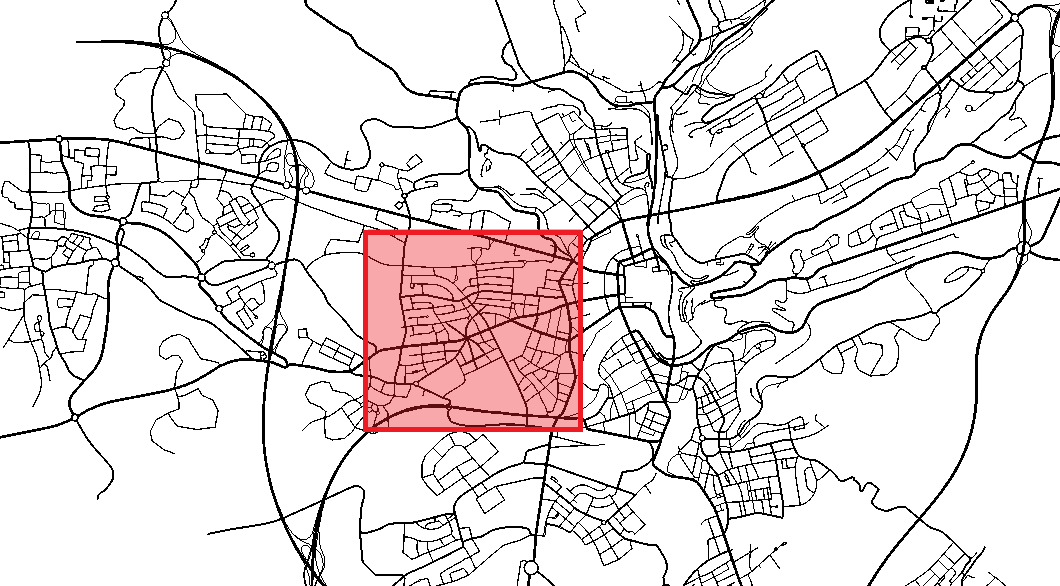
\includegraphics[width=1\columnwidth]{figures/LuxCity.png}
% \caption{Map and road grid of Luxembourg City center. The area within the red square corresponds to the region considered in our simulations.\vspace{-0.2in}}
% \label{fig:luxCity}
% \end{figure}
%
\begin{figure}[t!]
\centering
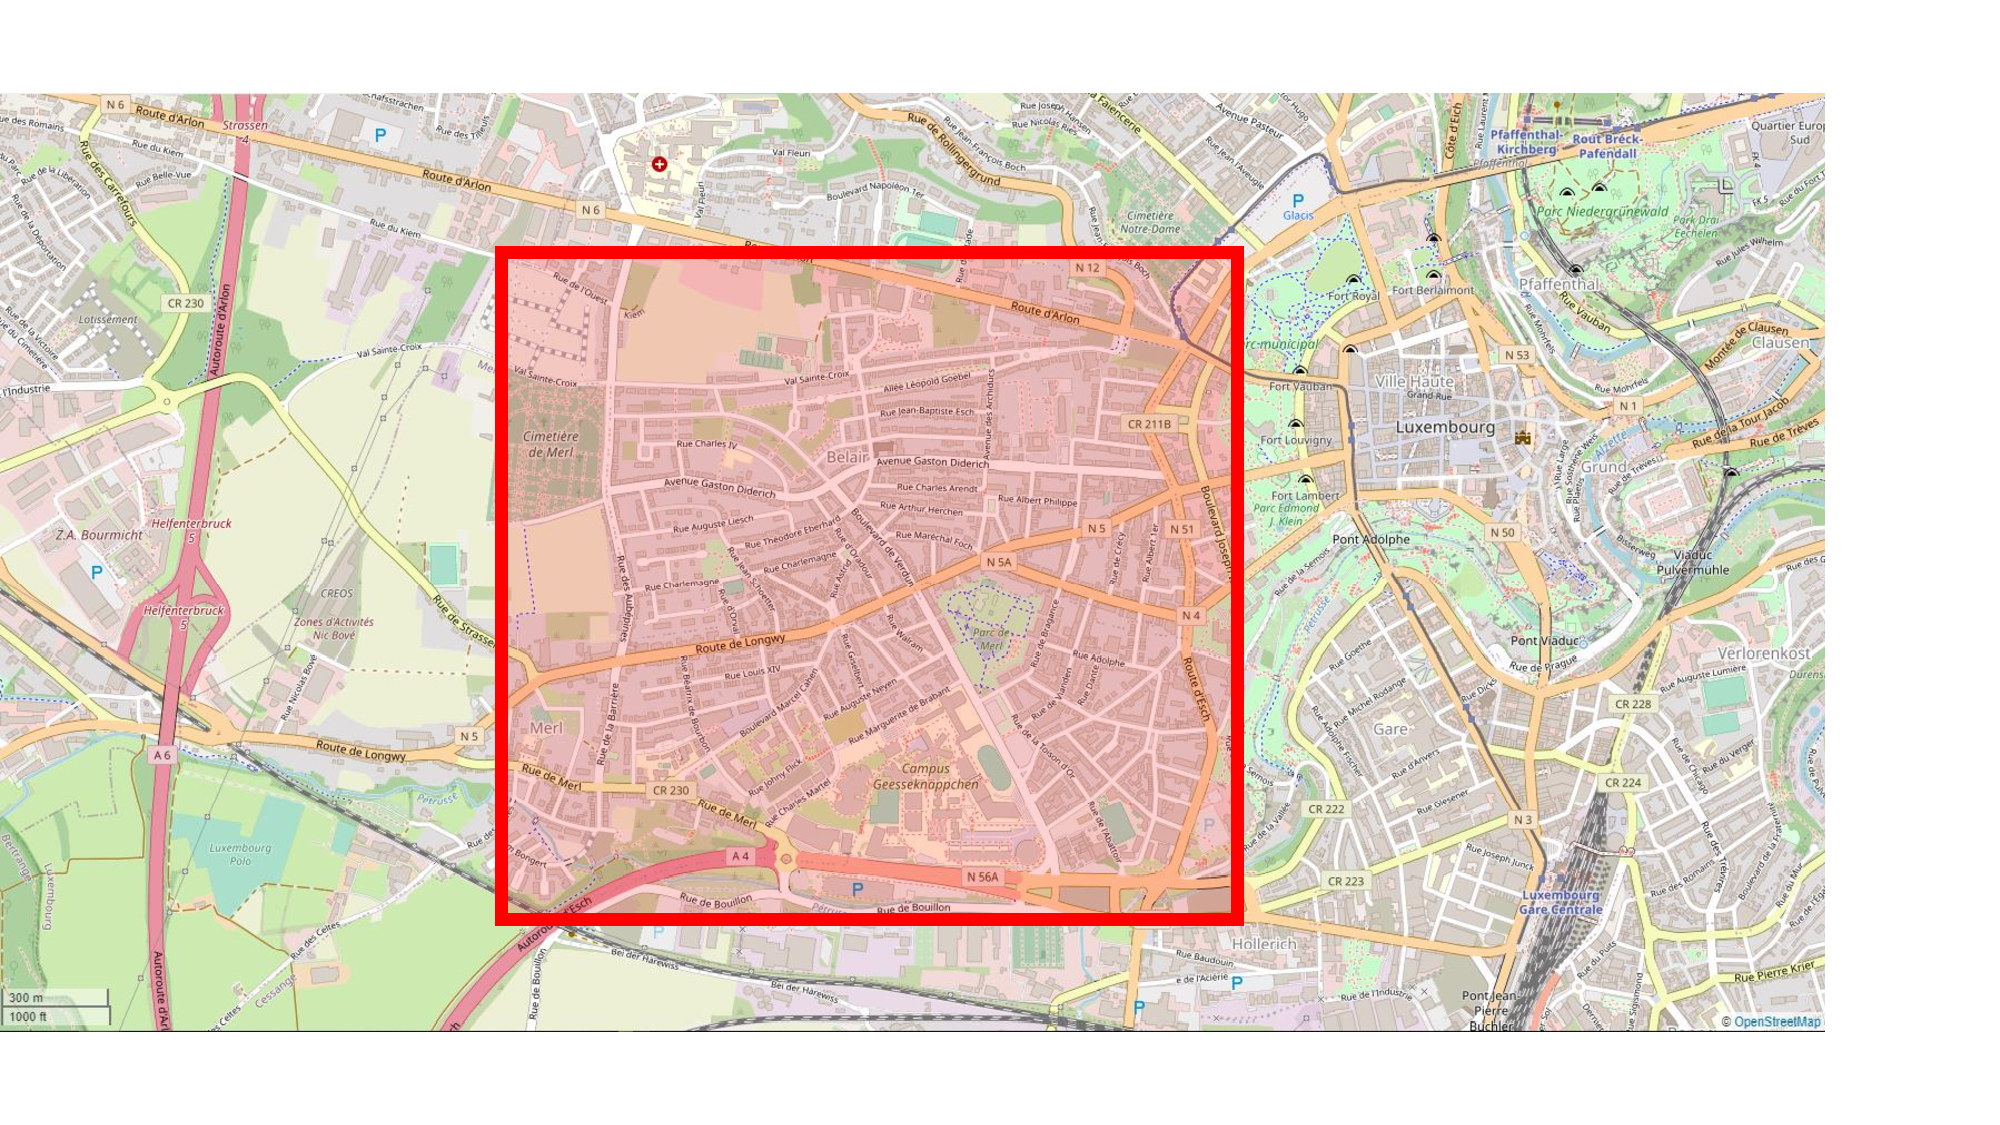
\includegraphics[width=1\columnwidth]{figures/lux_map_2.pdf}
\caption{Map and road grid of Luxembourg City center. The area within the red square corresponds to the region considered in our simulations.\vspace{-0.2in}}
\label{fig:luxCity}
\end{figure}

%
% \begin{figure}[b!]
% \centering
% 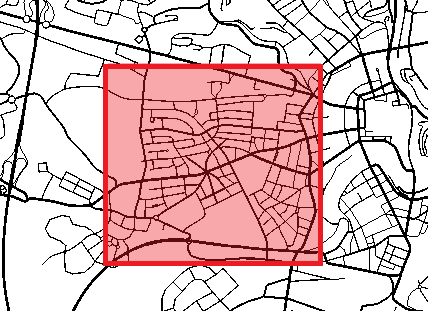
\includegraphics[width=1\columnwidth]{figures/LuxCitySmall.png}
% \caption{City center of the Luxembourg city. \vspace{-0.2in}}
% \label{fig:luxCity}
% \end{figure}

In this section we present the results of the numerical assessment of our framework for decentralized Gossip Learning.
In order to implement a realistic scenario in our simulation experiments, we adopted the dataset of the Luxembourg
SUMO Traffic (LuST) Scenario \cite{lux}, consisting in measurement-based vehicular traces over 24 hours from the city of Luxembourg, with a typical topology common in mid-size European cities, and with realistic traffic demand and mobility patterns. In particular, we considered a square region of side $1050$ m (\fref{fig:luxCity}) in the city center, within which we assumed that predictions of vehicle trajectories are required. We partitioned such region into $49$ square cells of side $150$ m, compatibly with the case in which each cell corresponds to the coverage area of a MEC-enabled small cell base station. As in many real scenarios, vehicular traffic flows exhibit non-stationary properties which might affect the accuracy of our GL trained models. In order to limit such effects of the variations of traffic flows over time, we observed the performance of our scheme over a time interval of one hour (specifically, from $6:30$ AM to $7:30$ AM, where vehicular traffic is sufficiently intense and stationary). Such time interval has been chosen to be, on one side, long enough to allow our training framework to progress substantially, but short enough for the average pattern of vehicular traffic flows not to vary significantly. In the given region, on average about $300$ vehicles are present at every time instant in the time interval considered, and every vehicle is in the range of about $60$ other vehicles, of which on average only half are in the exploitation phase and are thus able to act as clients.\\
%\footnote{\com{here I'd like exact numbers: memo for next time.}}\\
For implementing the simulations of opportunistic communications among vehicles, we adopted the Omnet++~\cite{Varga2010} framework, while Keras~\cite{chollet2018deep} was used for implementing our GL algorithm. We assumed vehicles sample their position in space every $5$ s, i.e. at rate comparable to that common in many present day car fleet management applications. Moreover, we assumed to require a prediction about a vehicle's position in $10$ seconds in the future. Such forecast horizon is of the same order of magnitude of those required in, e.g., predictive collision avoidance systems, or in MEC resource preallocation strategies. Our LSTM model input being composed by $24$ steps, it requires at least the last two minutes of the trajectory of a car in order to issue a trajectory prediction. 
%The goal of this work however is not reaching maximum accuracy or precision on the specific trajectory dataset. Rather, we wish to compare different methods to predict the vehicle trajectory in the next $10$ seconds. 
%We thus choose reasonable values for hyper-parameters, following indications in the literature. 
We considered each node performs model training over its entire local dataset, adopting a local batch size of $32$ data points (coherently with the indications in \cite{bengio2012practical} \cite{masters2018revisiting}, and a $10^{-3}$ learning rate, as suggested in ~\cite{geron2019hands}.\\
Given that in the scenario considered the average sojourn time of vehicles in the given region has been around $20$ minutes, after several experiments for each node we have chosen for the initialization phase a duration of about half of this time, i.e. $9$ m $30$ s. Indeed in the given setting such a duration is, on one side, short enough to have a substantial amount of nodes in the exploitation stage at each point in time (about $50\%$), and thus contributing to our collaborative training. On the other, it is long enough to have a substantial training set at each node, and thus to allow the collaborative training to progress at a reasonable rate within the residual sojourn time of each vehicle. Given the relatively short duration of the exploitation phase, we have experimentally verified that the periodic training of the local model instance on the local database during the exploitation phase has no significant impact on model accuracy. Note however that these considerations are strictly related to the characteristics of the chosen scenario, and specifically, to the size and shape of the given region, as well as the mean node speed. In order to perform a first evaluation of our approach, we have assumed that the tasks of model training, of computing a meta-model, and of exchanging a model are instantaneous, thus modeling the case in which the limiting factor of our training framework is given by the way in which training and meta-model computing task are implemented, rather than by their duration.\\       
% Therefore, each client initializes its weights randomly and trains the received models on the entire dataset. In the following we evaluate our algorithms with a fixed test set and short rolling test set.
% \footnote{\com{there should also be periodically, a training of the local model over its own data. This is important because due to the clean slate assumption, the dataset is small, and data accumultaed after the initialization phase may substantially improve the model. But how often? INCLUDED IT IN THE ALGO, BUT NUMERICALLY SAY THAT WE DID NOT DO IT BECAUSE DATASET WERE SMALL.}}
%%%%%%%%%%%%%%%%%%%%%%%%%%%%%
%In the following, we evaluate the performance of the proposed algorithms (DFed Avg, DFed Pow, and DFed MinLoss) through an online learning method. We update  models at each time interval when new data becomes available. We check the availability of data every five seconds.\\
\begin{figure}[t!]
\centering
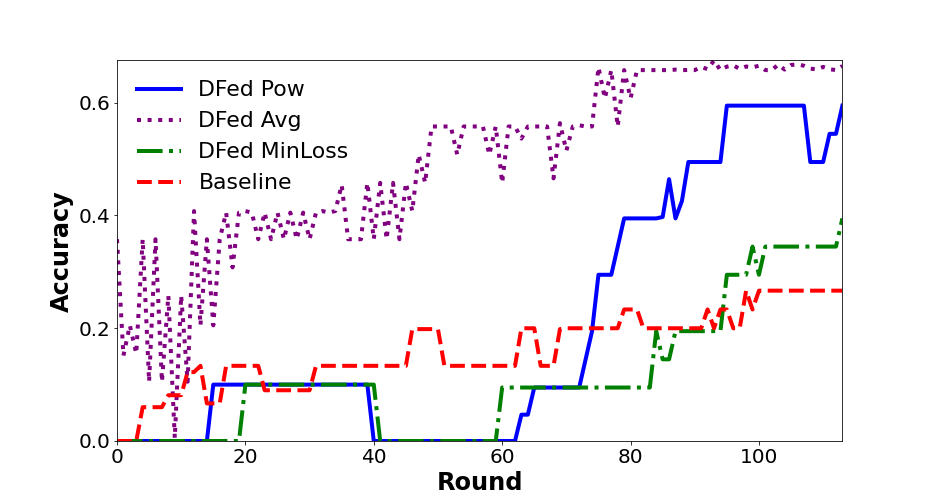
\includegraphics[width=1\columnwidth]{figures/accFixTest3.png} 
\caption{Mean accuracy versus iterations for our GL algorithm, for the three model merging schemes, and baseline model, with static test set, in the Luxembourg scenario.\vspace{-0.3in}}
\label{fig:accuracy}
\end{figure}
%
\begin{figure}[t!]
\centering
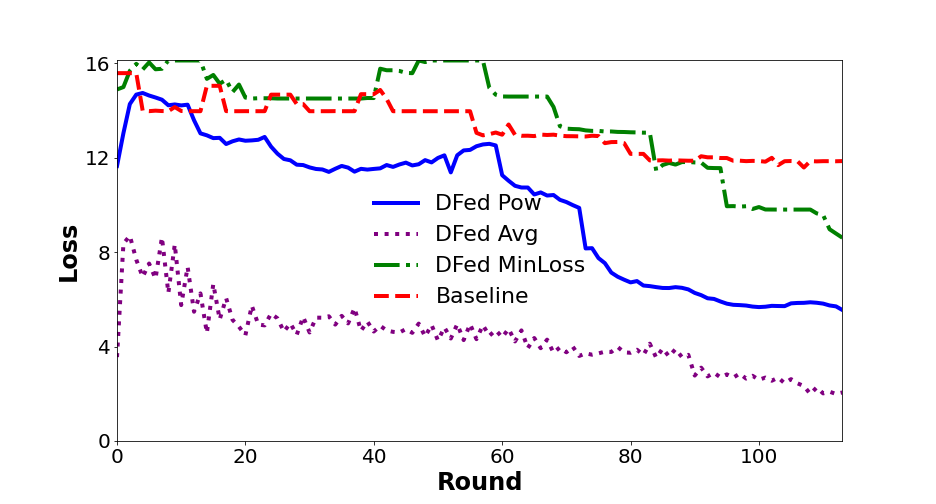
\includegraphics[width=1\columnwidth]{figures/lossFixedSet3.png} 
\caption{Mean loss versus iterations for our GL algorithm, for the three model merging schemes and baseline model with static test set, in the Luxembourg scenario. \vspace{-0.2in}}
\label{fig:loss}
\end{figure}
%
In order to assess the performance of the training process, the test set consisted in the data points of the trajectory of each vehicle within the last $5$ minutes of the vehicle's sojourn time within the given region. With such a choice for the test set (henceforth denoted as \textit{static}), at each point in time during the exploitation stage the evaluation is done on data points about parts of the map which are generally far from those in which the node is located. This holds also, on average, for the dataset of the client nodes. Finally, in order to better appreciate in what measure our collaborative training improves over purely local training, we have considered this latter approach as as a baseline, and we have characterized its performance.\\
\fref{fig:accuracy} and \fref{fig:loss} show accuracy and loss of our GL schemes, averaged over the $30$ cars in the area with longest sojourn time, for the static test set approach. As these figures show, one consequence of choosing a  static test set is that on average the initial loss is high (and the accuracy low) for all of the three meta-model building approaches, and sometimes even lower than the baseline. The figures also show that these parameters keep on improving steadily across the iterations of our GL training scheme.\\
These results show also that despite every node enters the scenario with an empty dataset, a substantial improvement in model accuracy can be achieved within a relatively small amount of rounds. The two plots indicate that, when vehicles spend a sufficiently large amount of time in the scenario, GL schemes can collaboratively train models which achieve a substantially better performance with respect to their initial, locally trained models, and over relatively short timespans.
Moreover, the plots \fref{fig:accuracy} and \fref{fig:loss} seem to suggest that, as expected, the main potential factor contributing to such improvement is the progress in model training, i.e. the gradual inclusion over time in the trained model of an ever larger amount of data about trajectories in the given region.\\ 
%This approach shows the performance of the trained model at the end of the vehicle's sojourn time, after that a sufficient amount of training cycles . In a sense thus, and thus it gives an idea of the best possible prediction performance achievable in such a clean-slate scenario.  
%The main performance metric in classification algorithms is accuracy, defined as the percentage of correctly classified outputs.
As for the relative performance of the three approaches to meta-model elaboration, \fref{fig:accuracy} and \ref{fig:loss} show that weighting each contribution to the meta-model based on the relative size of the local training set, outperforms approaches based on loss estimation. This might be due to the fact that while the validation set (over which loss is evaluated in the \textit{DFed Pow} and \textit{DFed MinLoss} approaches) consists in the last $V$ slots of a user's trajectory, and thus to a region of space very close to where the user will be in $h$ slots, the test set is relative to a portion of the user trajectory which is (generally, except for the final part of the vehicle's trajectory) far enough from the current vehicle position (and from where it will be) to make the performance over the validation set not indicative of the actual prediction accuracy of the model. I.e., as the model evolves constantly to adapt its performance to the specific prediction task and to the context in which the prediction is formulated, it would make more sense to take as test set data points which are as much as possible related to that same spatio-temporal context.\\
In order to address this issue, in a new set of experiments, at each time slot $t$ we have adopted as test set the data points relative to the time interval ${(i-l,i+h)}$ where $l$ is the length of the LSTM input (24 slots), and $h$ is the forecast horizon (equal to 2 slots in our experiments). This should allow a more relevant assessment of model performance, as it is performed over the same segment of a vehicle trajectory over which the prediction is performed. 
% In this experiment, after every communication round we evaluated the generated meta-model on the short size rolling test set. The test set at time interval $i$ is constituted of those samples associated to the time interval ${(i-l,i+h)}$ where $l$ is the time duration of the input sequence, and $h$ is the forecast horizon. In our case, $l$ corresponds to a total of 120 seconds of past samples, and $h$ corresponds to the next ten seconds from the current moment.\\
%
\begin{figure}[t!]
\centering
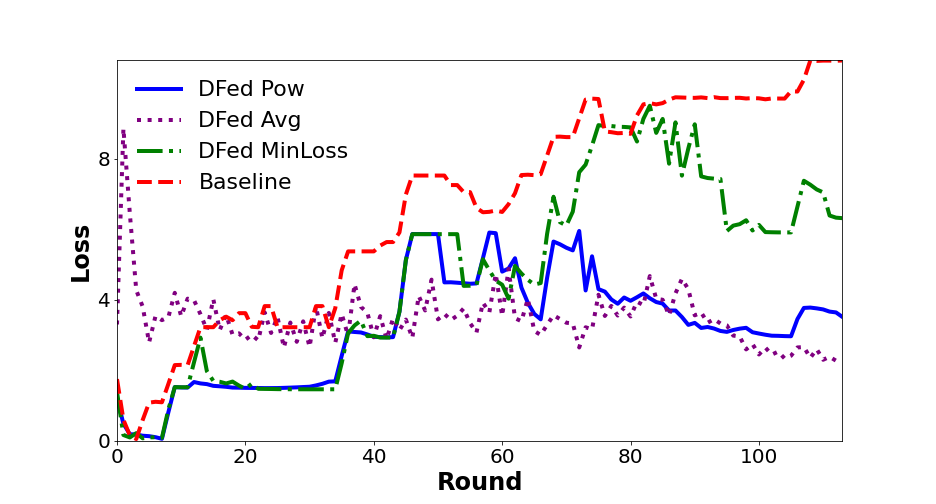
\includegraphics[width=1\columnwidth]{figures/lossShortRolling3.png} 
\caption{Mean loss versus iterations for our GL algorithm with a short size rolling test set, for the three model merging schemes, in the Luxembourg scenario. \vspace{-0.2in}}
\label{fig:lossS}
\end{figure}
%
\begin{figure}[t!]
\centering
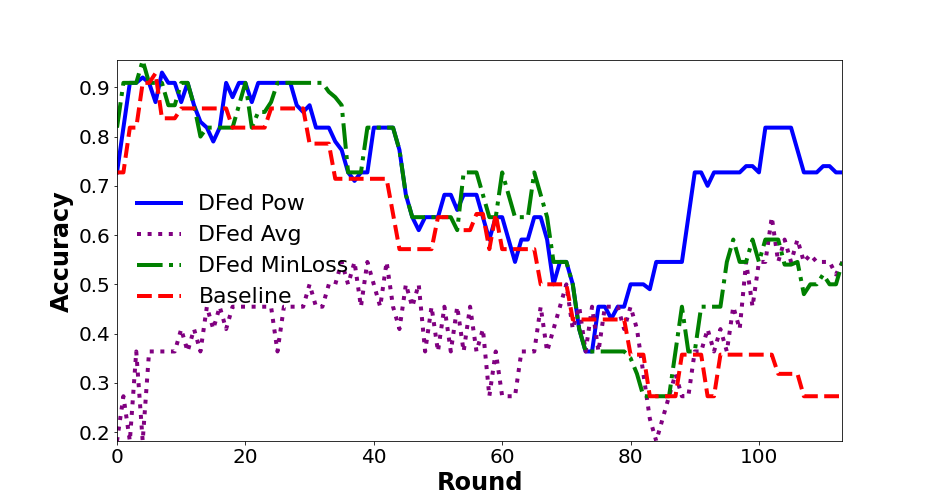
\includegraphics[width=1\columnwidth]{figures/accShortRoll3.png} 
\caption{Mean accuracy versus iterations for our GL algorithm with a short size rolling test set, for the three model merging schemes, in the Luxembourg scenario.\vspace{-0.3in}}
\label{fig:accuracyS}
\end{figure}
As \fref{fig:lossS} and \ref{fig:accuracyS} show, when assessed with a rolling test set the performance (both in terms of accuracy and of loss) of the models trained with our GL approach is generally less pessimistic than with a static test set. In addition, it remains approximately constant as the number of rounds increases, if not for fluctuations which are due to spatial in homogeneities in node density, in the structure of the road grid, and to bursts of nodes arriving and leaving the considered region. Moreover, in this setting the loss-based meta model building approaches perform generally better than the strategy based on the relative size of the local dataset of client nodes, with the DFed Pow performing slightly better than the DFed MinLoss. This is likely due to the fact that test set and validation set are now relative to contiguous regions of space and time interval, making loss measured over the validation set a more relevant indicator of the performance over the (rolling) test set. Note that improvement over the baseline becomes noticeable only after that a substantial amount of rounds has passed. This is due to the fact that the baseline algorithm has been obtained via training over a dataset which typically contains only a very limited number of cell transitions. Thus, it performs poorly whenever the node moves to another cell, an event whose likelihood grows with time, thus steadily worsening the performance of the purely locally trained model over time.  
% DFed Pow and DFed MinLoss show very similar behaviours in the first 70 rounds.
% DFed Avg from communication round 34 to 76 shows an almost constant performance, while DFed Pow and DFed MinLoss exhibit a performance deterioration.
% By looking in detail at datasets, we could see that in this time interval many nodes are moving to a new cell, and this makes the two algorithms worsen their performance in predicting the future trajectory. 
%are two. On one side, such improvement might reflect
%, i.e. as  nodes get closer to that part of the given region in which the test set data points are located. 
%These experiments show thus that the locality of the data on which models are trained plays a key role in improving the trained model over GL. That is, models trained through our GL scheme show significant improvements when the training set used for training (by the node itself, or by clients nodes in the GL scheme) belongs to the vicinity of the area by which the predicting node will pass in the near future.\\
%{\color{red}WE NEED TO SAY SOMETHING MORE ABOUT COMPARISONS.}

\vspace{-0.15in}
\section{Conclusions and future work}
\label{sec:Conclusion}
The preliminary results presented in this paper suggest that the performance of nodes with too small/poor datasets, or short sojourn times might be improved by having nodes with better models spread them opportunistically, and let other nodes use such received models as starting point for the GL algorithm. We thus plan on expanding the approach discussed in this paper with other forms of model exchanges among vehicles, which can better enable vehicles with short sojourn times and/or small datasets to contribute significatively to the model sharing scheme. Moreover, we plan on performing a thorough assessment of our algorithms on a variety of other vehicular scenarios, and to characterize their convergence properties.

%\com{@Mina: please review all cited works, making style uniform across all of them (not all have same level of detail), and adding capitalization wherever needed (you need to close the capitalized word within curly braces).}
%\vspace{-7pt}
% Currently, we are using real mobility scenarios in order to compare the results with our model. We would like to use this approach as support to localization system as GPS. Indeed, a vehicle could estimate its position though the position of another vehicle. 
%\vspace{-3pt}
%%%%%%%%%%%%%%%%%%%%%%%%%
% trigger a \newpage just before the given reference
% number - used to balance the columns on the last page
% adjust value as needed - may need to be readjusted if
% the document is modified later
%\IEEEtriggeratref{8}
% The "triggered" command can be changed if desired:
%\IEEEtriggercmd{\enlargethispage{-5in}}

% references section

% can use a bibliography generated by BibTeX as a .bbl file
% BibTeX documentation can be easily obtained at:
% http://mirror.ctan.org/biblio/bibtex/contrib/doc/
% The IEEEtran BibTeX style support page is at:
% http://www.michaelshell.org/tex/ieeetran/bibtex/
%\bibliographystyle{IEEEtran}
% argument is your BibTeX string definitions and bibliography database(s)
%\bibliography{IEEEabrv,../bib/paper}
%
% <OR> manually copy in the resultant .bbl file
% set second argument of \begin to the number of references
% (used to reserve space for the reference number labels box)



\bibliographystyle{IEEEtran}
\vspace{-12pt}
\bibliography{IEEEabrv,Bibliography}

\cleardoublepage


% that's all folks
\end{document}


